\documentclass[12pt]{article}
\pagenumbering{gobble}
\linespread{1.1}

\usepackage{amsfonts}
\usepackage{amsmath}
\usepackage{amssymb}
\usepackage{array}
\usepackage{fancyhdr}
\usepackage{mathrsfs}
\usepackage{mathtools}
\usepackage{parskip}
\usepackage{textcomp}
\usepackage[margin=1in,headheight=1in]{geometry}

\usepackage{tikz}
\usetikzlibrary{animations}
\usetikzlibrary{arrows.meta}
\usetikzlibrary{calc}
\usetikzlibrary{shapes.geometric}

\graphicspath{ {./images/} }

\newcommand{\contradiction}{
    \ensuremath{{\Rightarrow\mspace{-2mu}\Leftarrow}}
}

% bracket commands
\newcommand{\angleb}[1]{\left\langle#1\right\rangle} % <>
\newcommand{\vertb}[1]{\left\vert#1\right\vert}      % ||
\newcommand{\bracks}[1]{\left[#1\right]}             % []
\newcommand{\braces}[1]{\left\{#1\right\}}           % {}
\newcommand{\parens}[1]{\left(#1\right)}             % ()

% set aliases
\newcommand{\N}{\mathbb{N}}
\newcommand{\Z}{\mathbb{Z}}
\newcommand{\Q}{\mathbb{Q}}
\newcommand{\R}{\mathbb{R}}

\newcommand{\derv}[2]{\dfrac{d#1}{d#2}}
\newcommand{\e}{\varepsilon}
\newcommand{\di}{\,/\,}

\newcommand{\lm}[1]{\displaystyle\lim_{#1}}

\begin{document}
\pagestyle{fancy}
\fancyhead{}
\fancyhead[L]{Alex Agruso}
\fancyhead[R]{Topology Writing 10}

\normalsize

\section*{Part I}

\begin{itemize}
    \item [a.)] The resulting shape is depicted below.

    \begin{center}
        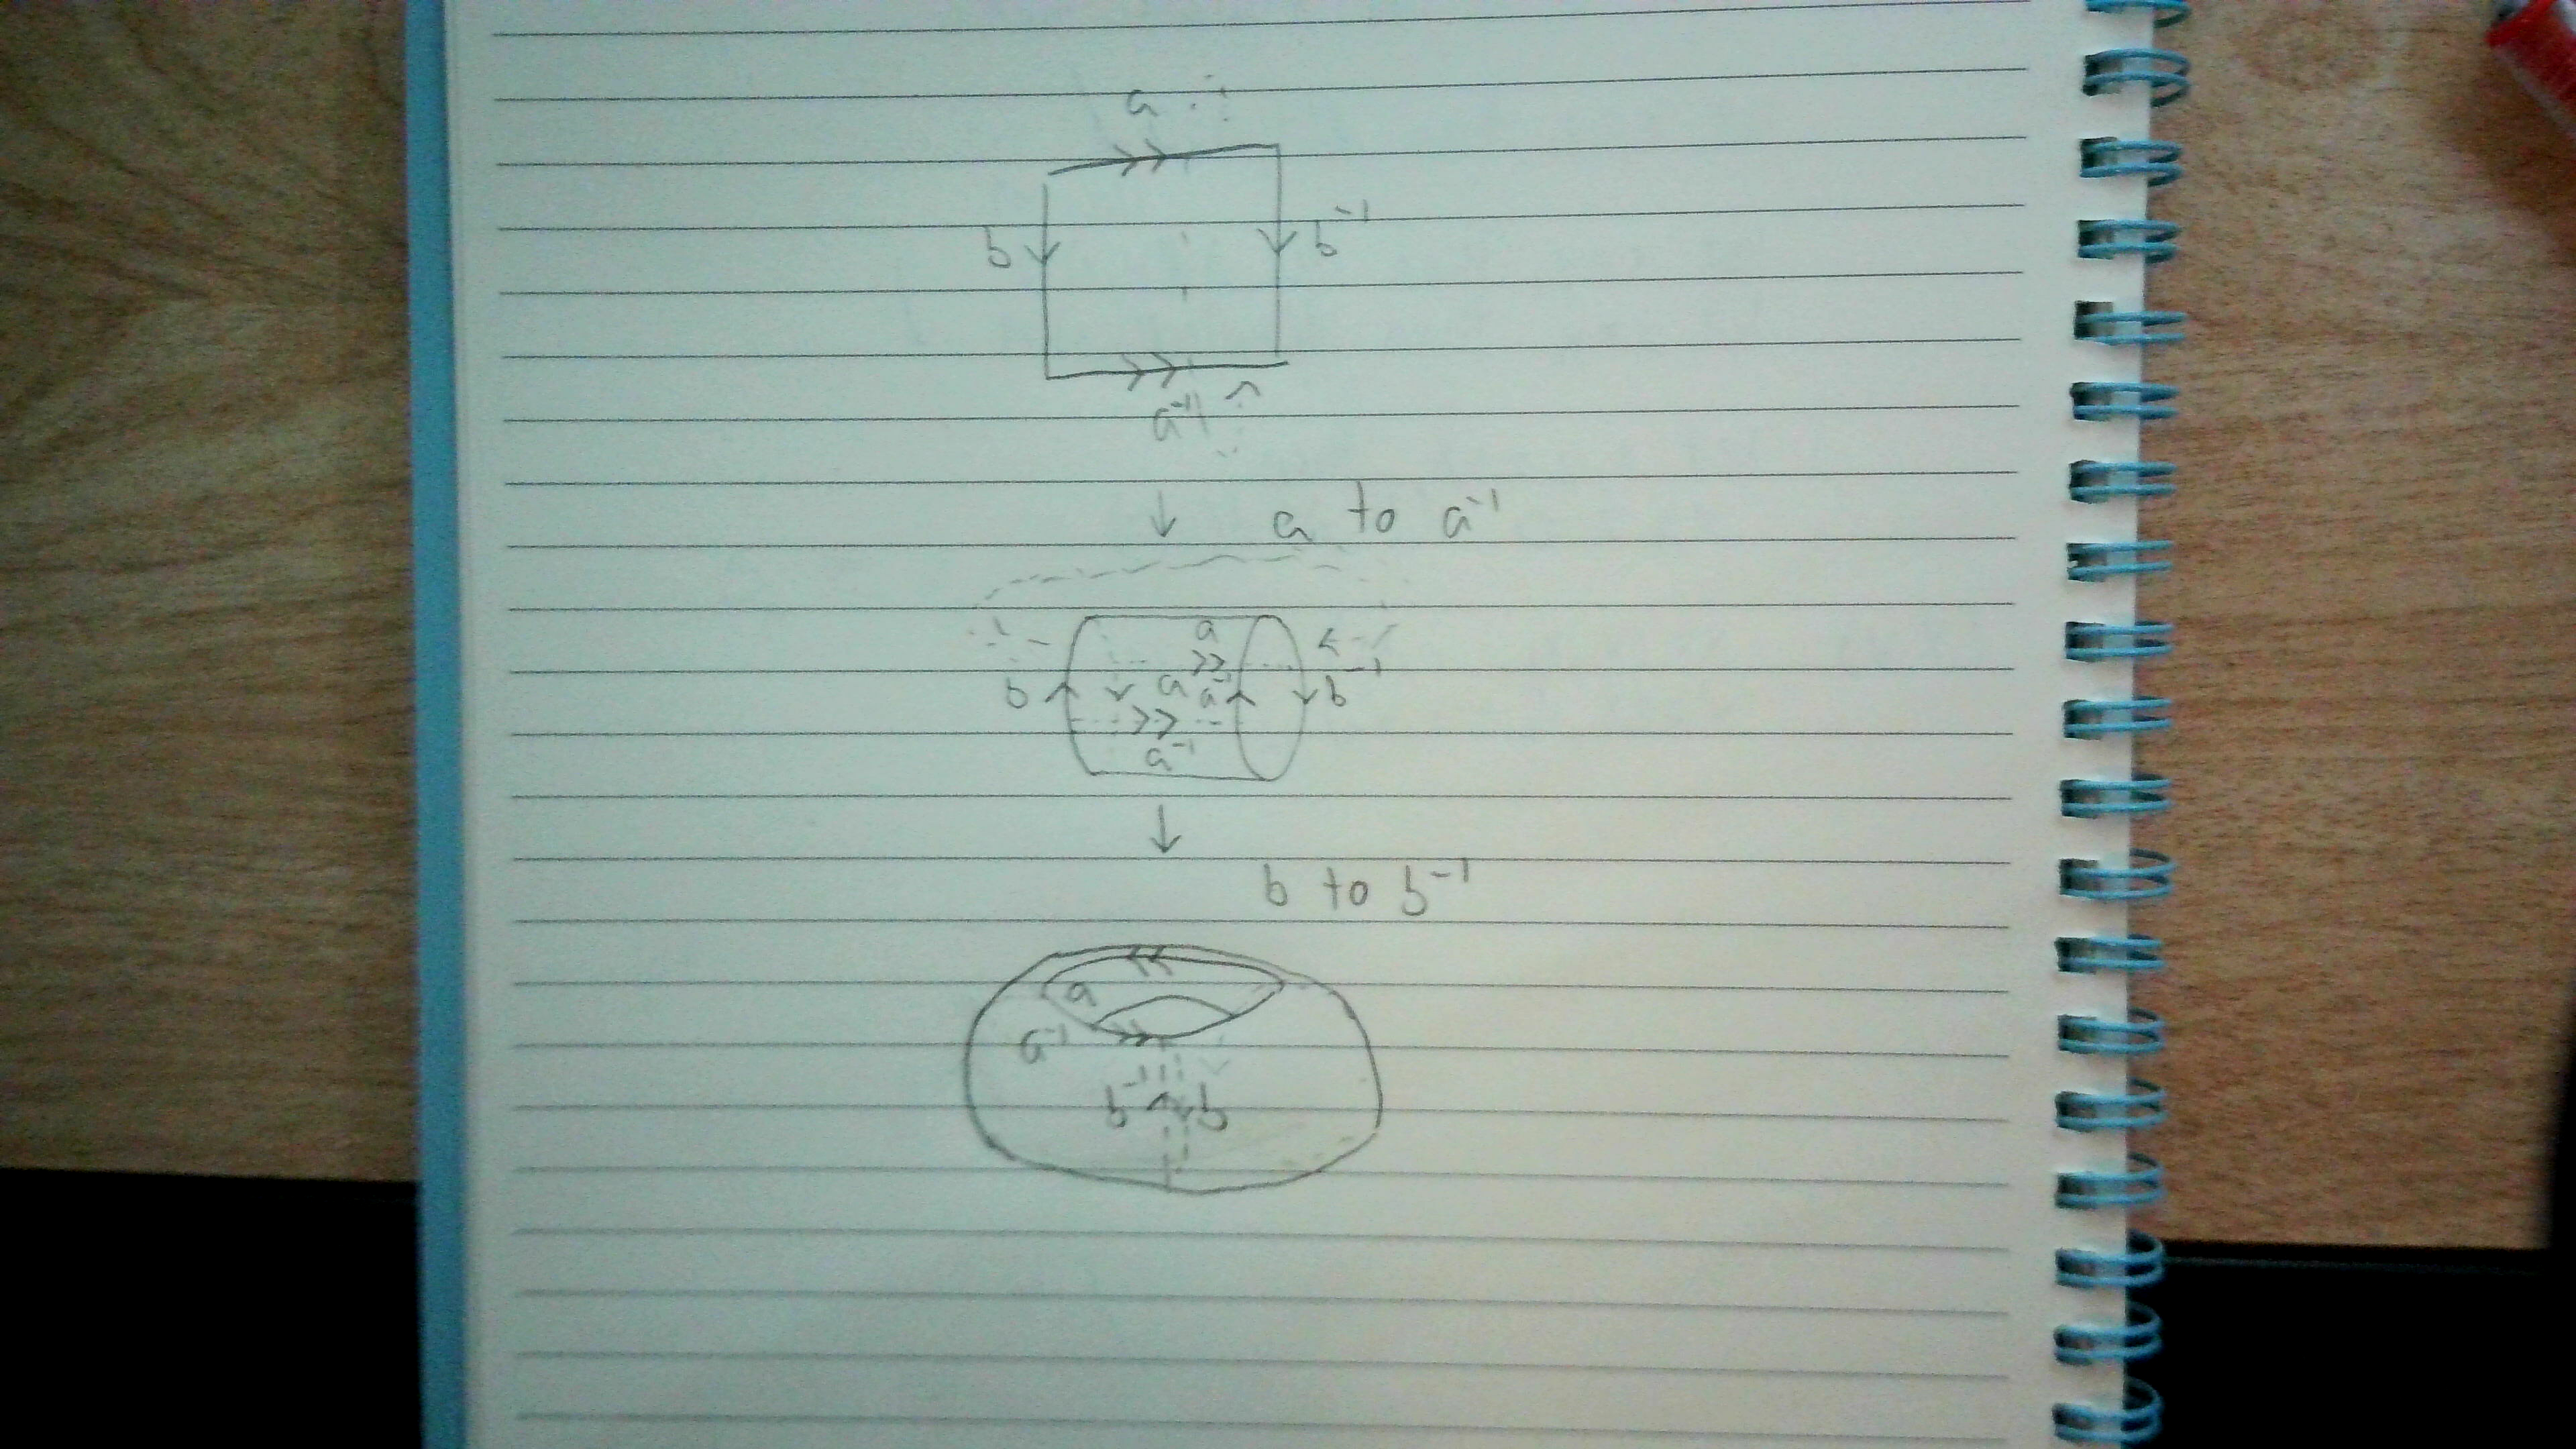
\includegraphics[scale=0.1]{images/Question1.jpeg}
    \end{center}

    \item [b.)] We could define an equivalence relation on two points $(x,y),(x',y')$ in $[0,1]\times[0,1]$ that says two points are equivalent if they either take the form $(x,0),(x',1)$ or $(0,y),(1,y')$ where $x=x'$ and $y=y'$.
\end{itemize}

\pagebreak
\section*{Part II}

\begin{itemize}
    \item [a.)] The resulting shape is depicted below.
    \begin{center}
        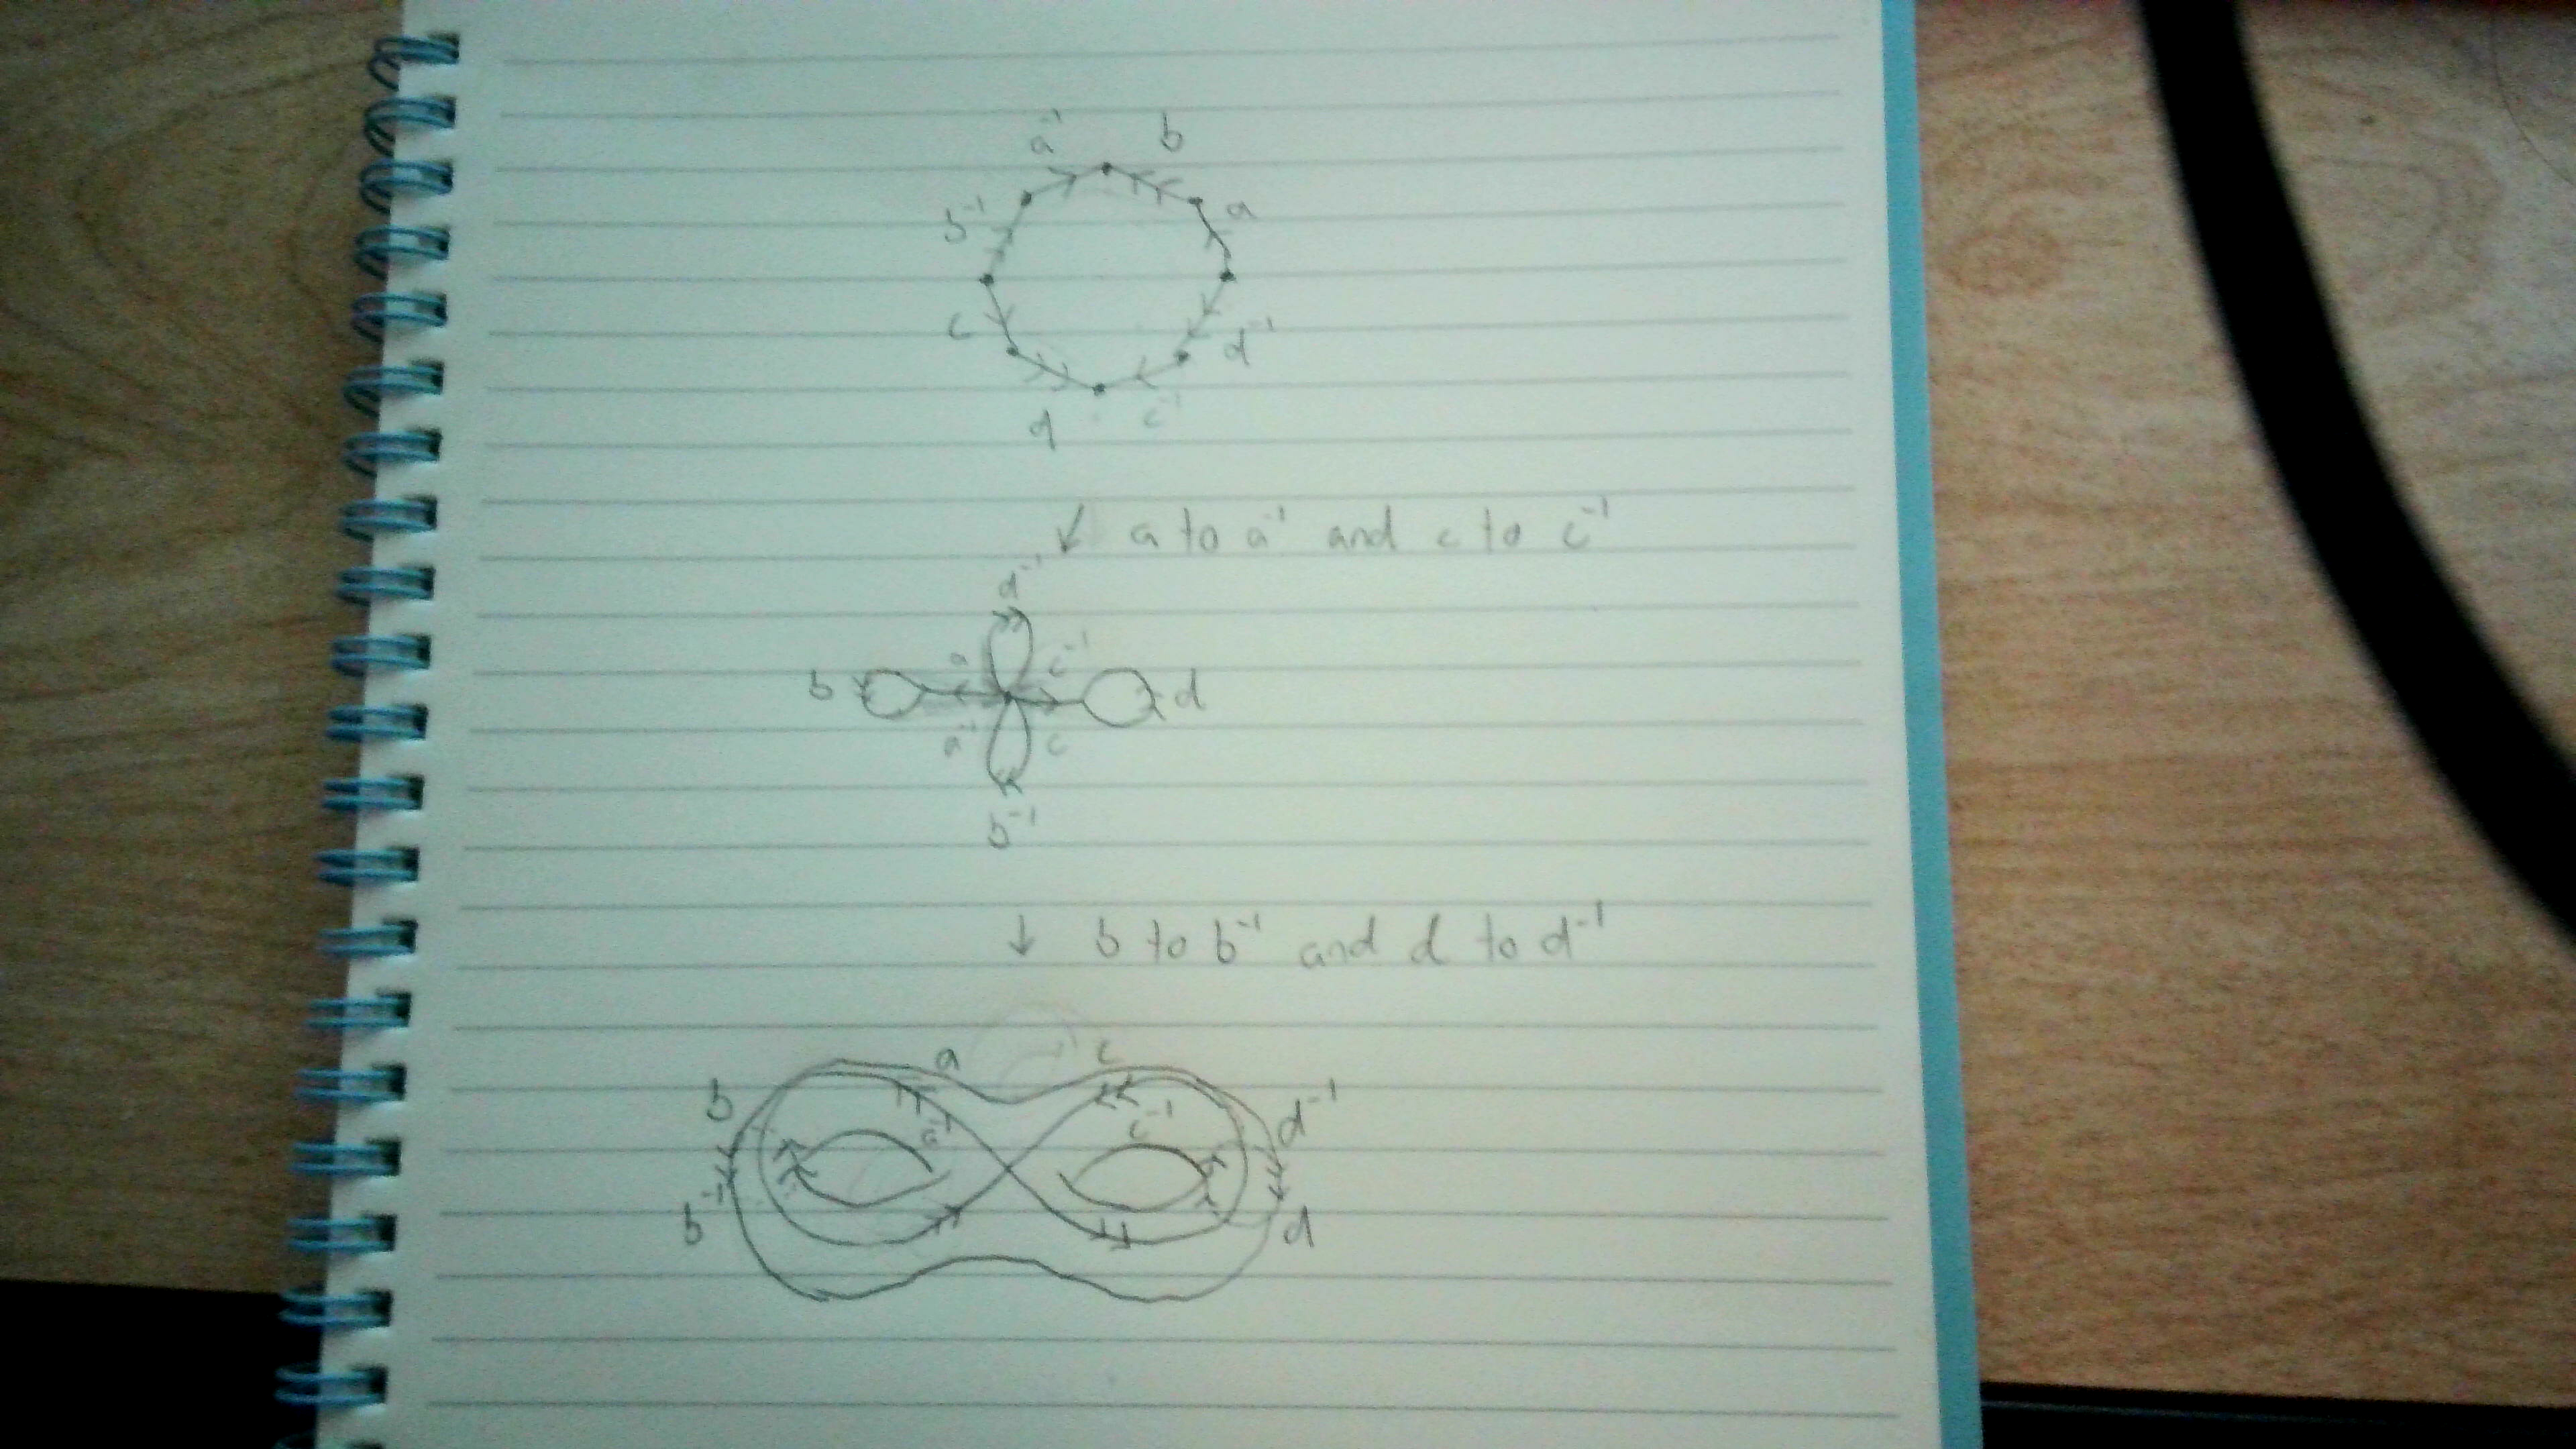
\includegraphics[scale=0.1]{images/Question2.jpeg}
    \end{center}

    \item [b.)] Take two complementary edges, e.g. $a$ and $a^{-1}$, and draw a perpendicular line through the midpoint of the edge between them. We can now say two points are equivalent if they are the reflection of one another across the previously determined line.
\end{itemize}

\end{document}
